\chapter{Jantung dan Paru-paru Selama Usaha}\label{ch:g10:heart-lungs-effort}

Larilah menaiki empat lantai tangga lalu berhenti di puncaknya. Dadamu
naik turun --- empat puluh embusan tiap menit alih-alih dua belas,
masing-masing tiga kali lebih dalam --- dan jantungmu berdegup pada
seratus tujuh puluh. Tidak ada satu pun tentang tangga itu yang menuntut
kamu memutuskan hal ini; tubuhmu mengaturnya, dalam hitungan sekon,
karena otot pada \cref{ch:g10:exercise-and-energy} sedang menuntut
oksigen sepuluh kali lebih banyak daripada semenit sebelumnya. Bab ini
membahas sistem pengantarannya --- paru-paru, jantung, pembuluh darah
--- dan bagaimana keluarannya dilipatgandakan ketika usaha dimulai.

\section{Ventilasi}

\begin{definition}[Ventilasi]\label{def:g10:heart-lungs-effort:ventilation}
Yang disebut \emph{ventilasi paru}\index{ventilasi} adalah volume udara
yang dipindahkan masuk dan keluar paru-paru tiap menit: volume satu
embusan napas (\emph{volume tidal}) dikalikan jumlah embusan tiap menit
(\emph{frekuensi napas}). Dalam keadaan istirahat, sekitar \qty{0.5}{L}
dua belas sampai lima belas kali tiap menit: \qtyrange{6}{8}{L/min}. Di
dalam paru-paru udaranya mencapai sekitar 300 juta
\emph{alveolus}\index{alveolus}, yaitu kantong berdinding tipis yang
terbungkus kapiler, tempat oksigen berpindah ke dalam darah dan karbon
dioksida keluar darinya.
\end{definition}

\begin{proposition}[Ventilasi selama olahraga]\label{prop:g10:heart-lungs-effort:vent-exercise}
Selama olahraga, volume tidal dan frekuensinya sama-sama naik: orang
dewasa yang bugar dapat menghirup \qty{2.5}{L} empat puluh kali tiap
menit, yaitu \qty{100}{L/min} atau lebih, lima belas kali nilai
istirahatnya. Kenaikannya mulai dalam sekon pertama usahanya, sebelum
ada perubahan apa pun dalam darahnya, dan mantap pada aras yang
sebanding dengan oksigen yang sedang dipakai.
\end{proposition}
\admitted

\begin{omfigure}
\begin{tikzpicture}
\begin{axis}[
  width=0.9\linewidth, height=6.2cm,
  axis x line=bottom, axis y line=left,
  xmin=0, xmax=40, ymin=0, ymax=6.5,
  xlabel={waktu (s)}, ylabel={volume paru-paru (L)},
  xlabel style={font=\small, at={(axis description cs:0.5,-0.1)}, anchor=north},
  ylabel style={font=\small},
  tick label style={font=\small}, xtick={0,10,20,30,40}, ytick={0,1,2,3,4,5,6},
  clip=false,
]
\addplot[thick, omDef, smooth, samples=200, domain=0:16]
  {2.7 + 0.25*sin(deg(2*pi*x/4))};
\addplot[thick, omDef] coordinates {(16,2.7) (18,2.95) (21,5.7) (25,5.7) (30,1.2) (33,1.2) (35,2.7)};
\addplot[thick, omDef, smooth, samples=100, domain=35:40]
  {2.7 + 0.25*sin(deg(2*pi*(x-35)/4))};
\draw[dashed, gray] (axis cs:0,1.2) -- (axis cs:40,1.2);
\draw[dashed, gray] (axis cs:0,5.7) -- (axis cs:40,5.7);
\draw[dashed, gray] (axis cs:0,2.45) -- (axis cs:18,2.45);
\draw[dashed, gray] (axis cs:0,2.95) -- (axis cs:18,2.95);
\draw[<->, omThm] (axis cs:38,1.2) -- (axis cs:38,5.7);
\node[font=\small, anchor=west, omThm] at (axis cs:38.4,3.5) {kapasitas};
\node[font=\small, anchor=west, omThm] at (axis cs:38.4,3.1) {vital};
\draw[<->] (axis cs:8,2.45) -- (axis cs:8,2.95);
\node[font=\small, anchor=south] at (axis cs:8,3.0) {volume tidal, \qty{0.5}{L}};
\node[font=\small, anchor=north] at (axis cs:20,1.1) {volume sisa};
\node[font=\small, anchor=south, align=center] at (axis cs:23,5.75) {inspirasi\\ maksimal};
\node[font=\small, anchor=north, align=center] at (axis cs:31.5,1.1) {};
\end{axis}
\end{tikzpicture}

{\small Sebuah spirogram: volume udara dalam paru-paru terhadap waktu.
Bernapas tenang memindahkan \qty{0.5}{L} tiap embusan di sekitar aras
tengah; inspirasi maksimal yang disusul ekspirasi maksimal menyapu
kapasitas vitalnya, sekitar \qty{4.5}{L}; \qty{1.2}{L} yang tidak
pernah dapat diembuskan adalah volume sisanya.}
\end{omfigure}

\begin{example}[Membaca sebuah spirogram]\label{ex:g10:heart-lungs-effort:spirogram}
Pada gambarnya, empat embusan napas memakan \qty{16}{s}: 15 embusan
tiap menit sebesar \qty{0.5}{L}, jadi \qty{7.5}{L/min}. Sapuan
maksimalnya berjalan dari \qty{5.7}{L} turun ke \qty{1.2}{L}: kapasitas
vital \qty{4.5}{L}. Volume tidal \qty{2.5}{L} selama olahraga memakai
lebih dari separuh kapasitas itu, dan itulah sebabnya bernapas berat
terasa seperti itu.
\end{example}

\begin{omfigure}
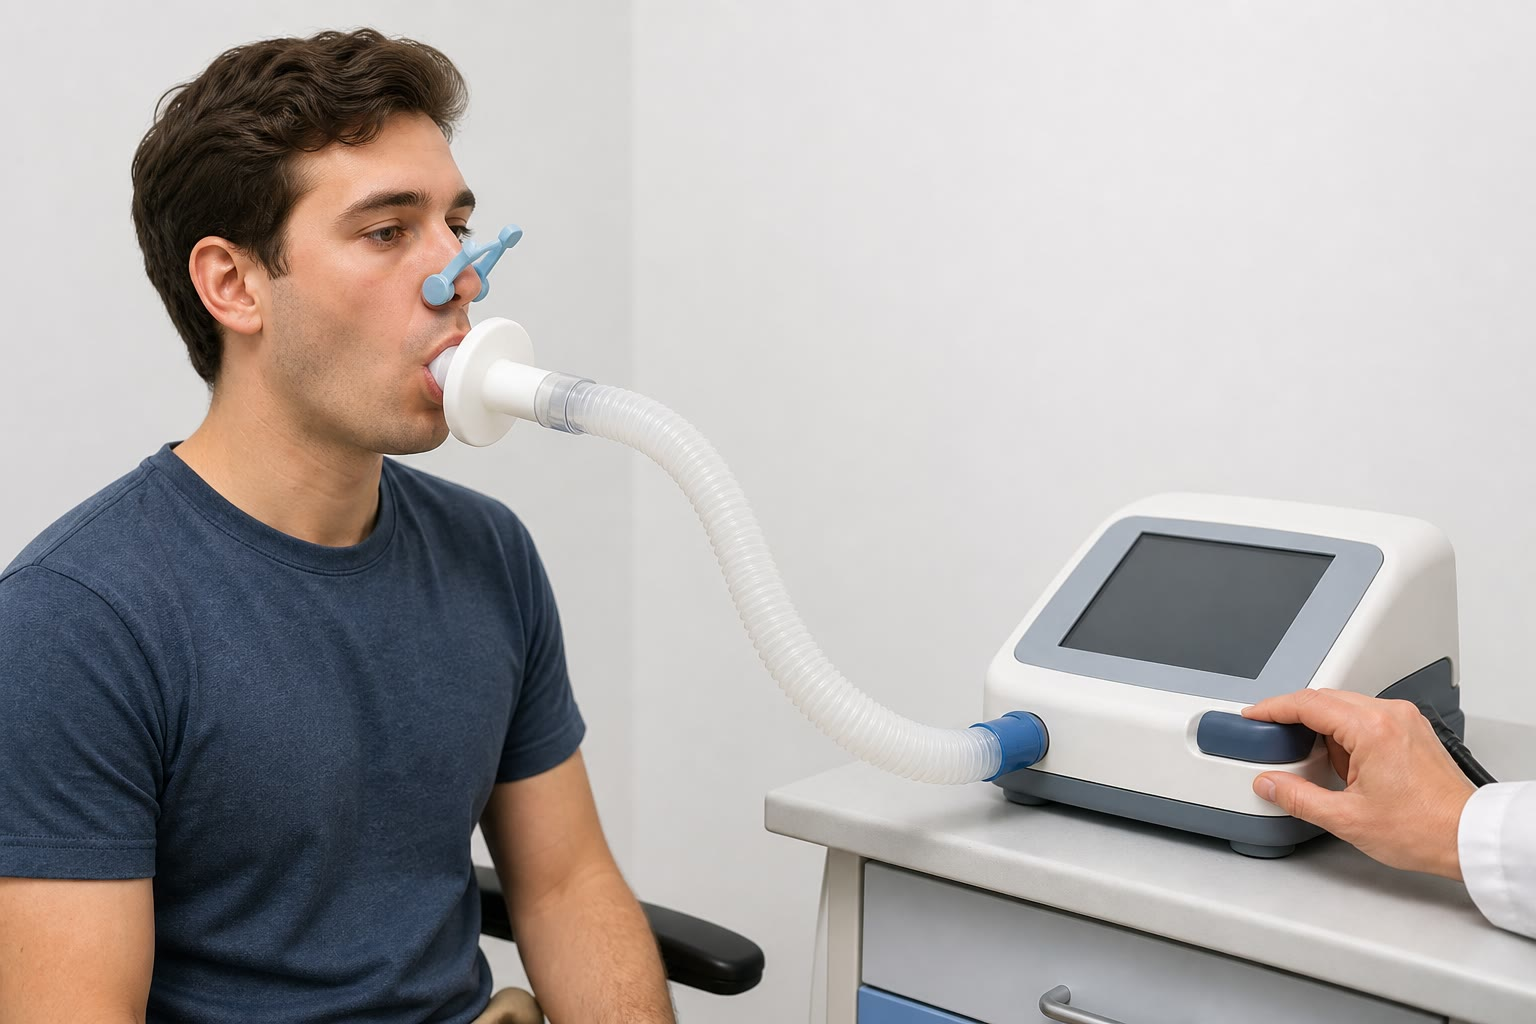
\includegraphics[width=0.58\linewidth]{images/book2/ai/g10-lungs-spirometer.jpg}

{\small Mengukur volume paru-paru: subjeknya bernapas lewat corong
mulut ke dalam spirometer, dengan hidung terjepit, dan alatnya merekam
volume tiap embusan napasnya.}
\end{omfigure}

\section{Jantung dan kedua peredarannya}

\begin{definition}[Curah jantung]\label{def:g10:heart-lungs-effort:output}
Jantung adalah pompa ganda berisi empat ruang. Sisi kanannya menerima
darah yang kembali dari organ dan mengirimkannya ke paru-paru
(\emph{peredaran paru}); sisi kirinya menerimanya kembali dari
paru-paru dan mengirimkannya ke organ (\emph{peredaran sistemik}).
Katup di antara ruangnya dan pada pintu keluarnya membuat alirannya
searah. Yang disebut \emph{curah jantung}\index{curah jantung} $Q$
adalah volume darah yang dipompa tiap sisi tiap menit: volume yang
disemburkan tiap denyut, yaitu \emph{volume sekuncup} $V_s$, dikalikan
\emph{frekuensi denyut jantung} $f$,
\[
Q = f \times V_s .
\]
Dalam keadaan istirahat, $70$ denyut tiap menit sebesar \qty{70}{mL}:
sekitar \qty{5}{L/min} --- seluruh volume darahnya sekali tiap menit.
\end{definition}

\begin{omfigure}
\begin{tikzpicture}[>=Stealth, font=\small,
  ch/.style={draw, thick, rounded corners, minimum width=1.9cm, minimum height=1.0cm, align=center},
  org/.style={draw, thick, rounded corners, minimum width=2.6cm, minimum height=1.0cm, align=center}]
  \node[org, fill=omDef!15] (lungs) at (3.5,3.6) {paru-paru};
  \node[ch, fill=omDef!25] (ra) at (0.7,1.2) {serambi\\ kanan};
  \node[ch, fill=omDef!25] (rv) at (0.7,0) {bilik\\ kanan};
  \node[ch, fill=omThm!20] (la) at (6.3,1.2) {serambi\\ kiri};
  \node[ch, fill=omThm!20] (lv) at (6.3,0) {bilik\\ kiri};
  \node[org, fill=omThm!12] (org) at (3.5,-2.8) {otot dan\\ organ lainnya};
  \draw[->, thick, omDef] (ra) -- (rv);
  \draw[->, thick, omDef, rounded corners=6pt] (rv.west) -- (-1.55,0) -- (-1.55,3.6) -- (lungs.west);
  \node[anchor=east, align=right, omDef] at (-1.7,2.4) {arteri\\ paru};
  \draw[->, thick, omThm, rounded corners=6pt] (lungs.east) -- (8.6,3.6) -- (8.6,1.2) -- (la.east);
  \node[anchor=west, align=left, omThm] at (8.75,2.4) {vena\\ paru};
  \draw[->, thick, omThm] (la) -- (lv);
  \draw[->, thick, omThm, rounded corners=6pt] (lv.east) -- (8.6,0) -- (8.6,-2.8) -- (org.east);
  \node[anchor=west, omThm] at (8.75,-1.4) {aorta};
  \draw[->, thick, omDef, rounded corners=6pt] (org.west) -- (-2.3,-2.8) -- (-2.3,1.2) -- (ra.west);
  \node[anchor=east, omDef] at (-2.45,-1.4) {vena};
  \node[font=\small, anchor=north, text width=3.2cm, align=center] at (3.5,-3.6) {oksigen keluar, $\mathrm{CO_2}$ masuk};
  \node[font=\small, anchor=south, text width=3.2cm, align=center] at (3.5,4.2) {oksigen masuk, $\mathrm{CO_2}$ keluar};
  \draw[thick, dashed, gray] (3.5,2.5) -- (3.5,-1.9);
\end{tikzpicture}

{\small Peredaran ganda. Biru: darah yang miskin oksigen, yang dipompa
jantung kanan ke paru-paru. Merah: darah yang kaya oksigen, yang
dipompa jantung kiri ke organ. Kedua sisinya berdenyut bersama dan
memompa volume yang sama tiap menit.}
\end{omfigure}

\begin{proposition}[Curah jantung selama olahraga]\label{prop:g10:heart-lungs-effort:output-exercise}
Selama olahraga frekuensi denyut jantung naik seiring daya yang
diberikan, sampai maksimum kira-kira $220$ dikurangi umurnya dalam
tahun, dan volume sekuncupnya ikut naik, sekitar separuh pada orang tak
terlatih dan lebih banyak pada yang terlatih. \omterm{def:g10:heart-lungs-effort:output}{Curah jantung} orang
dewasa muda berjalan dari \qty{5}{L/min} dalam keadaan istirahat ke
\qtyrange{20}{25}{L/min} pada usaha maksimal, dan ke \qty{35}{L/min}
atau lebih pada juara olahraga ketahanan, yang volume sekuncupnya dapat
melampaui \qty{180}{mL}.
\end{proposition}
\admitted

\begin{omfigure}
\begin{tikzpicture}
\begin{axis}[
  width=0.86\linewidth, height=5.8cm,
  axis x line=bottom, axis y line=left,
  xmin=0, xmax=320, ymin=0, ymax=210,
  xlabel={daya mekanis (W)}, ylabel={denyut jantung (tiap min), volume sekuncup (mL)},
  xlabel style={font=\small, at={(axis description cs:0.5,-0.12)}, anchor=north},
  ylabel style={font=\small},
  tick label style={font=\small},
  xtick={0,50,100,150,200,250,300}, ytick={0,50,100,150,200},
  legend style={at={(0.5,-0.3)}, anchor=north, legend columns=3, font=\small, draw=none},
  clip=false,
]
\addplot[thick, omThm, mark=*, mark size=1.5pt] coordinates
  {(0,70) (50,95) (100,120) (150,145) (200,170) (250,190) (300,198)};
\addplot[thick, omDef, mark=square*, mark size=1.5pt] coordinates
  {(0,70) (50,90) (100,105) (150,112) (200,115) (250,115) (300,115)};
\addplot[thick, omMeth, dashed, mark=triangle*, mark size=1.8pt] coordinates
  {(0,4.9) (50,8.6) (100,12.6) (150,16.2) (200,19.6) (250,21.9) (300,22.8)};
\legend{denyut jantung, volume sekuncup, curah (L/min)}
\end{axis}
\end{tikzpicture}

{\small Frekuensi denyut jantung, volume sekuncup dan \omterm{def:g10:heart-lungs-effort:output}{curah jantung}
seorang berumur dua puluh tahun pada daya yang meningkat. Volume
sekuncupnya mendatar pada usaha sedang; di atas itu curahnya naik lewat
frekuensinya saja, dan frekuensinya sendiri mendatar mendekati $220 - 20 = 200$.}
\end{omfigure}

\begin{example}[Curah pada \qty{200}{W}]\label{ex:g10:heart-lungs-effort:output200}
Dari gambarnya: $f = 170$ tiap menit, $V_s = \qty{115}{mL}$, sehingga
$Q = 170 \times 0.115 \approx \qty{19.6}{L/min}$: empat kali curah
istirahatnya. Jantungnya memindahkan seluruh volume darah tubuhnya
empat kali tiap menit.
\end{example}

\section{Mengantarkan darah ke tempat yang memerlukannya}

\begin{proposition}[Pembagian ulang aliran darah]\label{prop:g10:heart-lungs-effort:redistribution}
Dalam keadaan istirahat ototnya menerima sekitar seperlima \omterm{def:g10:heart-lungs-effort:output}{curah
jantung}; usus, hati dan ginjalnya mengambil separuhnya. Selama olahraga
berat, arteri kecil otot yang bekerja melebar dan arteri usus serta
ginjalnya menyempit: ototnya lalu menerima lebih dari empat perlima
curah yang dirinya sendiri sudah berlipat empat --- sekitar
\qty{20}{L/min} alih-alih \qty{1}{L/min}, dua puluh kali lebih banyak.
Bagian otaknya dijaga tetap dalam ukuran mutlak, dan bagian kulitnya
naik untuk membawa kalornya pergi.
\end{proposition}
\admitted

\begin{omfigure}
\begin{tikzpicture}
\begin{axis}[
  xbar stacked, bar width=15pt,
  width=0.86\linewidth, height=3.8cm,
  axis x line=bottom, axis y line=left,
  xmin=0, xmax=25, xlabel={aliran darah (L/min)},
  xlabel style={font=\small, at={(axis description cs:0.5,-0.3)}, anchor=north},
  symbolic y coords={istirahat, olahraga maksimal},
  ytick=data, tick label style={font=\small},
  enlarge y limits=0.5,
  legend style={at={(0.5,-0.65)}, anchor=north, legend columns=5, font=\small, draw=none},
]
\addplot[fill=omThm!50, draw=omThm] coordinates {(1.0,istirahat) (20.5,olahraga maksimal)};
\addplot[fill=omProp!50, draw=omProp] coordinates {(2.5,istirahat) (0.9,olahraga maksimal)};
\addplot[fill=omDef!50, draw=omDef] coordinates {(0.75,istirahat) (0.75,olahraga maksimal)};
\addplot[fill=gray!40, draw=gray] coordinates {(0.5,istirahat) (1.2,olahraga maksimal)};
\addplot[fill=omMeth!50, draw=omMeth] coordinates {(0.25,istirahat) (0.65,olahraga maksimal)};
\legend{otot, usus dan ginjal, otak, kulit, lainnya}
\end{axis}
\end{tikzpicture}

{\small Ke mana \omterm{def:g10:heart-lungs-effort:output}{curah jantungnya} pergi, dalam keadaan istirahat
(\qty{5}{L/min}) dan pada olahraga maksimal (\qty{24}{L/min}). Bagian
ototnya berjalan dari seperlima menjadi lebih dari empat perlima;
otaknya menjaga \qty{0.75}{L/min}-nya sepanjang waktu.}
\end{omfigure}

\begin{proposition}[Pengantaran dan pengambilan oksigen]\label{prop:g10:heart-lungs-effort:extraction}
Tiap liter darah arteri membawa sekitar \qty{200}{mL} oksigen, yang
hampir seluruhnya terikat pada hemoglobin \omterm{def:g10:cells-common-unit:cell}{sel} darah merah. Dalam
keadaan istirahat organnya menyingkirkan sekitar \qty{50}{mL} dari tiap
liter; selama olahraga otot yang bekerja menyingkirkan sampai
\qty{150}{mL}, tiga kali lebih banyak. Oksigen yang terpakai tiap menit
adalah \omterm{def:g10:heart-lungs-effort:output}{curah jantung} dikalikan jumlah yang disingkirkan tiap liter ---
sehingga kenaikan lima kali lipat pada curahnya dan kenaikan tiga kali
lipat pada pengambilannya bersama-sama memberi kenaikan lima belas kali
lipat pada konsumsi oksigen \cref{ch:g10:exercise-and-energy}.
\end{proposition}
\admitted

\begin{example}[Anggaran oksigennya diperiksa]\label{ex:g10:heart-lungs-effort:fick}
Istirahat: \qty{5}{L/min} $\times$ \qty{50}{mL/L} $= \qty{250}{mL/min}$,
yaitu konsumsi istirahatnya. Usaha maksimal seorang murid terlatih:
\qty{23}{L/min} $\times$ \qty{150}{mL/L} $= \qty{3.45}{L/min}$ --- yaitu
$\dot V\!\mathrm{O_2}$maks \qty{50}{mL/min} tiap kilogram bagi
\qty{69}{kg}, persis angka bab sebelumnya.
\end{example}

\section{Bagaimana tanggapannya dikendalikan}

\begin{proposition}[Kendali saraf dan hormon]\label{prop:g10:heart-lungs-effort:control}
Jantung dan otot pernapasan dijalankan oleh pusat saraf di dasar
otaknya. Dua perangkat saraf mencapai jantungnya: satu memperlambatnya,
yang aktif dalam keadaan istirahat; satu mempercepatnya dan menguatkan
tiap denyutnya. Pada awal olahraga, perintah otak kepada ototnya
disalin ke pusat itu --- jantungnya mempercepat diri dalam satu atau dua
denyut --- dan pengindra dalam otot serta sendinya melaporkan
gerakannya. Lalu, seiring berlanjutnya olahraga, pengindra dalam
arterinya mengukur karbon dioksida dan keasaman darahnya dan menyetel
\omterm{def:g10:heart-lungs-effort:ventilation}{ventilasi} serta denyut jantungnya agar tetap dekat ke nilai
istirahatnya. Kelenjar adrenalnya menambahkan hormon
\emph{adrenalin}\index{adrenalin}, yang memperkuat percepatannya dan
melebarkan arteri ototnya.
\end{proposition}
\begin{proof}[Bukti percobaan]
Memotong saraf pelambat seekor hewan menaikkan denyut jantung
istirahatnya dari 70 menjadi sekitar 100; merangsangnya menghentikan
jantungnya. Merangsang saraf pemercepatnya melipatduakan denyutnya.
Seseorang yang diberi tahu untuk bersiap berusaha memperlihatkan denyut
jantung yang naik sebelum bergerak; subjek yang menghirup udara yang
diperkaya karbon dioksida meningkatkan \omterm{def:g10:heart-lungs-effort:ventilation}{ventilasinya} dalam satu menit,
dan subjek yang karbon dioksida darahnya dijaga tetap secara buatan
selama olahraga tetap meningkatkannya pada awal gerakannya --- kedua
mekanismenya, yaitu antisipasi dan koreksi, sama-sama nyata.
\end{proof}

\begin{method}[Menghitung pengantaran oksigen]\label{met:g10:heart-lungs-effort:compute}
\begin{enumerate}
  \item \omterm{def:g10:heart-lungs-effort:ventilation}{Ventilasi}: volume tidal $\times$ frekuensi. Hanya sekitar 70\%
        tiap embusan napas yang mencapai \omterm{def:g10:heart-lungs-effort:ventilation}{alveolusnya}; sisanya mengisi
        saluran udaranya.
  \item \omterm{def:g10:heart-lungs-effort:output}{Curah jantung}: $Q = f \times V_s$, dalam liter tiap menit jika
        $V_s$ dalam liter.
  \item Oksigen yang terpakai tiap menit: $Q \times$ (oksigen yang
        disingkirkan tiap liter darah).
  \item Aliran ke sebuah organ: bagiannya dari $Q$. Bandingkan aliran
        mutlaknya, bukan bagiannya --- bagian yang lebih kecil dari
        curah yang lebih besar dapat berarti darah yang lebih banyak.
  \item Periksa: konsumsinya tidak dapat melampaui
        $\dot V\!\mathrm{O_2}$maks, dan $f$ tidak dapat melampaui
        sekitar $220 - $ umurnya.
\end{enumerate}
\end{method}

\begin{remark}[Di mana batasnya terletak]\label{rem:g10:heart-lungs-effort:limit}
\omterm{def:g10:heart-lungs-effort:ventilation}{Ventilasi} dapat melampaui \qty{150}{L/min} dan darah yang meninggalkan
paru-paru masih hampir jenuh pada usaha maksimal: paru-parunya bukan
lehernya. Volume sekuncupnyalah lehernya: ia menetapkan berapa banyak
darah, dan dengan demikian berapa banyak oksigen, yang diantar tiap
denyut. Latihan ketahanan memperbesar jantung dan volume sekuncupnya
--- dan itulah sebabnya jantung istirahat yang terlatih berdenyut pada
45 alih-alih 70 untuk \qty{5}{L/min} yang sama, dan sebabnya
$\dot V\!\mathrm{O_2}$maks naik seiring latihan.
\end{remark}

\section{Latihan}

\begin{exercise}[$\star$]\label{exo:g10:heart-lungs-effort:1}
Hitung \omterm{def:g10:heart-lungs-effort:ventilation}{ventilasi} seseorang yang menghirup \qty{0.6}{L} empat belas kali
tiap menit; lalu \omterm{def:g10:heart-lungs-effort:ventilation}{ventilasi} orang yang sama yang menghirup \qty{2.2}{L}
tiga puluh lima kali tiap menit.
\end{exercise}

\begin{exercise}[$\star$]\label{exo:g10:heart-lungs-effort:2}
Rumuskan \omterm{def:g10:heart-lungs-effort:output}{curah jantung} dan berikan rumusnya. Hitung curahnya untuk
denyut jantung 65 tiap menit dan volume sekuncup \qty{75}{mL}.
\end{exercise}

\begin{exercise}[$\star$]\label{exo:g10:heart-lungs-effort:3}
Telusuri jalur satu \omterm{def:g10:cells-common-unit:cell}{sel} darah merah dari serambi kanan kembali ke
serambi kanan, dengan menyebutkan ruang dan kedua peredarannya.
\end{exercise}

\begin{exercise}[$\star$]\label{exo:g10:heart-lungs-effort:4}
Dari gambar spirogramnya, sebutkan volume tidal, kapasitas vital dan
volume sisanya.
\end{exercise}

\begin{exercise}[$\star$]\label{exo:g10:heart-lungs-effort:5}
Berapa denyut jantung maksimal anak berumur 16 tahun? Berumur 60 tahun?
\end{exercise}

\begin{exercise}[$\star\star$]\label{exo:g10:heart-lungs-effort:6}
Dari gambar denyut jantungnya, hitung \omterm{def:g10:heart-lungs-effort:output}{curah jantung} pada \qty{100}{W}
dan pada \qty{300}{W}, serta faktor di antara keduanya.
\end{exercise}

\begin{exercise}[$\star\star$]\label{exo:g10:heart-lungs-effort:7}
Dalam keadaan istirahat usus dan ginjalnya menerima 50\% dari
\qty{5}{L/min}; pada olahraga maksimal, 4\% dari \qty{24}{L/min}.
Hitung kedua alirannya. Mana yang berubah lebih besar, bagiannya atau
aliran mutlaknya?
\end{exercise}

\begin{exercise}[$\star\star$]\label{exo:g10:heart-lungs-effort:8}
Seorang subjek punya \omterm{def:g10:heart-lungs-effort:output}{curah jantung} \qty{18}{L/min} dan ototnya
menyingkirkan \qty{140}{mL} oksigen tiap liter. Hitung konsumsi
oksigennya. Apakah ia mendekati batas atas seorang murid terlatih?
\end{exercise}

\begin{exercise}[$\star\star$]\label{exo:g10:heart-lungs-effort:9}
Mengapa aliran darah otaknya tetap \qty{0.75}{L/min} sementara aliran
ususnya dipotong dua pertiga selama olahraga? Pikirkan apa yang dapat
ditahan tiap organnya.
\end{exercise}

\begin{exercise}[$\star\star$]\label{exo:g10:heart-lungs-effort:10}
Seorang pesepeda terlatih punya denyut jantung istirahat 42 dan curah
istirahat \qty{5}{L/min}. Hitung volume sekuncupnya dan bandingkan
dengan volume sekuncup orang yang tak terlatih.
\end{exercise}

\begin{exercise}[$\star\star$]\label{exo:g10:heart-lungs-effort:11}
Jelaskan mengapa denyut jantungnya mulai naik sebelum langkah pertama
sebuah lomba, dan apa yang akan terjadi pada pelari yang kendalinya
hanya bekerja lewat pengindraan karbon dioksida darah.
\end{exercise}

\begin{exercise}[$\star\star\star$]\label{exo:g10:heart-lungs-effort:12}
Dua subjek mencapai denyut jantung maksimal yang sama, yaitu 195. Yang
satu punya volume sekuncup maksimal \qty{110}{mL}, yang lain
\qty{160}{mL}. Dengan pengambilan oksigen yang sama sebesar
\qty{150}{mL/L}, hitung \omterm{def:g10:exercise-and-energy:vo2max}{konsumsi oksigen maksimal} keduanya, dan
sebutkan apa yang diramalkan \cref{rem:g10:heart-lungs-effort:limit}
tentang riwayat latihan keduanya.
\end{exercise}

\begin{exercise}[$\star\star\star$]\label{exo:g10:heart-lungs-effort:13}
Udara mengandung 21\% oksigen. Seorang subjek berventilasi
\qty{100}{L/min} pada usaha maksimal dan memakai \qty{3.5}{L/min}
oksigen. Berapa bagian oksigen yang dihirupnya yang sungguh dipakainya?
Apa yang dikerjakan sisanya?
\end{exercise}

\begin{exercise}[$\star\star\star$]\label{exo:g10:heart-lungs-effort:14}
Sebuah obat menghalangi saraf pemercepat dan pengaruh \omterm{prop:g10:heart-lungs-effort:control}{adrenalin} pada
jantungnya, sehingga denyut jantungnya terbatas pada 110. Ramalkan
pengaruhnya pada \omterm{def:g10:heart-lungs-effort:output}{curah jantung} saat usaha maksimal, pada
$\dot V\!\mathrm{O_2}$maks, dan pada apa yang dapat dilakukan pasiennya.
\end{exercise}

\begin{exercise}[$\star\star\star$]\label{exo:g10:heart-lungs-effort:15}
Seseorang di tempat tinggi punya darah arteri yang membawa
\qty{150}{mL} oksigen tiap liter alih-alih \num{200}. Dengan \omterm{def:g10:heart-lungs-effort:output}{curah
jantung} maksimal yang sama dan pengambilan yang sama sebesar 75\%
oksigen yang diantarkan, hitung kehilangan $\dot V\!\mathrm{O_2}$maks
dalam persen. Usulkan satu penyesuaian yang dibuat tubuhnya dalam
pekan-pekan berikutnya.
\end{exercise}

\section{Soal: Uji Beban Jantung}

\begin{problem}[{Soal akhir pekan --- sebuah uji olahraga oleh dokter
jantung: denyut jantung, volume sekuncup, ventilasi dan pengambilan
oksigen yang diukur pada daya yang meningkat, dan pelipatgandaan yang
dicapainya bersama-sama}]
\label{pb:g10:heart-lungs-effort:1}
Tom, 17 tahun, bermassa \qty{68}{kg}, mengayuh sepeda laboratorium
sementara denyut jantung, \omterm{def:g10:heart-lungs-effort:ventilation}{ventilasi} dan udara embusannya direkam. Hasilnya:

\begin{center}
\begin{tabular}{lccccc}
daya (W) & 0 & 75 & 150 & 225 & 300 \\ \hline
denyut jantung (tiap min) & 62 & 105 & 140 & 175 & 198 \\
volume sekuncup (mL) & 72 & 100 & 116 & 120 & 120 \\
volume tidal (L) & 0.5 & 1.2 & 1.8 & 2.3 & 2.6 \\
embusan napas tiap min & 13 & 18 & 24 & 32 & 44 \\
$\mathrm{O_2}$ yang disingkirkan tiap liter darah (mL) & 52 & 90 & 120 & 145 & 155 \\
\end{tabular}
\end{center}

\medskip
\noindent\textbf{Bagian I --- Jantungnya.}
\begin{enumerate}
  \item Hitung \omterm{def:g10:heart-lungs-effort:output}{curah jantung} Tom pada tiap dayanya.
  \item Dengan faktor berapa curahnya naik pada \qty{300}{W}? Bagian
        mana dari faktor itu yang berasal dari frekuensinya dan bagian
        mana dari volume sekuncupnya?
  \item Di atas daya berapa volume sekuncupnya berhenti naik? Apa
        sendirian yang menaikkan curahnya di luar itu?
  \item Bandingkan denyut jantung maksimal Tom dengan aturan praktisnya.
  \item Curah istirahatnya sekitar \qty{4.5}{L/min}. Jika volume
        darahnya \qty{5}{L}, berapa lama satu putaran penuh memakan
        waktu dalam keadaan istirahat, dan pada \qty{300}{W}?
\end{enumerate}

\medskip
\noindent\textbf{Bagian II --- Paru-parunya.}
\begin{enumerate}[resume]
  \item Hitung \omterm{def:g10:heart-lungs-effort:ventilation}{ventilasinya} pada tiap dayanya.
  \item Dengan faktor berapa \omterm{def:g10:heart-lungs-effort:ventilation}{ventilasinya} naik pada \qty{300}{W}? Mana
        dari kedua faktornya, volume atau frekuensi, yang menyumbang
        lebih banyak?
  \item Kapasitas vital Tom \qty{5.0}{L}. Berapa bagiannya yang dipakai
        tiap embusan napas pada \qty{300}{W}?
  \item \omterm{def:g10:heart-lungs-effort:ventilation}{Ventilasinya} naik dengan faktor yang lebih besar daripada \omterm{def:g10:heart-lungs-effort:output}{curah
        jantungnya}. Apakah ini berarti paru-parunya membatasi
        kemampuannya? Pakai \cref{rem:g10:heart-lungs-effort:limit}.
  \item Hanya 70\% tiap embusan napas yang mencapai \omterm{def:g10:heart-lungs-effort:ventilation}{alveolusnya}. Hitung
        \omterm{def:g10:heart-lungs-effort:ventilation}{ventilasi} \omterm{def:g10:heart-lungs-effort:ventilation}{alveolusnya} dalam keadaan istirahat dan pada \qty{300}{W}.
\end{enumerate}

\medskip
\noindent\textbf{Bagian III --- Oksigennya.}
\begin{enumerate}[resume]
  \item Hitung konsumsi oksigen Tom pada tiap dayanya, dari \omterm{def:g10:heart-lungs-effort:output}{curah
        jantung} dan oksigen yang disingkirkan tiap liternya.
  \item Nyatakan nilainya pada \qty{300}{W} dalam mililiter tiap menit
        tiap kilogram. Apakah itu sebuah $\dot V\!\mathrm{O_2}$maks,
        dan milik subjek macam apa?
  \item Dengan faktor berapa konsumsinya naik dari keadaan istirahat ke
        \qty{300}{W}? Pecahlah menjadi faktor dari jantungnya dan
        faktor dari pengambilannya.
  \item Dengan \qty{20}{kJ} tiap liter oksigen, hitung daya
        \omterm{def:g10:cell-metabolism:metabolism}{metabolismenya} pada \qty{300}{W} dan efisiensi ototnya (daya
        mekanis dibagi daya \omterm{def:g10:cell-metabolism:metabolism}{metabolisme} di atas keadaan istirahat).
  \item Gambarkan, atau lukiskan, konsumsi oksigen terhadap daya
        mekanisnya. Apakah linear? Di mana batas atasnya?
\end{enumerate}

\medskip
\noindent\textbf{Bagian IV --- Kendali dan putusannya.}
\begin{enumerate}[resume]
  \item Denyut jantung Tom mencapai 75 ketika ia duduk menunggu ujinya
        dimulai. Jelaskan.
  \item Pada \qty{300}{W} darah arterinya masih 95\% jenuh dengan
        oksigen. Apa yang diberitahukannya tentang pertukaran di
        \omterm{def:g10:heart-lungs-effort:ventilation}{alveolusnya}, dan tentang di mana batas
        $\dot V\!\mathrm{O_2}$maks-nya terletak?
  \item Dokter jantungnya mencatat bahwa ototnya kini menerima sekitar
        \qty{20}{L/min} darah. Berapa bagian curahnya itu, dan ke mana
        sisa pembagian istirahatnya pergi?
  \item Setelah enam bulan latihan, volume sekuncup maksimal Tom
        \qty{140}{mL} pada frekuensi maksimal dan pengambilan yang
        sama. Hitung $\dot V\!\mathrm{O_2}$maks barunya.
  \item Nyatakan hasilnya: ketiga bilangan (jantung, pengambilan,
        \omterm{def:g10:heart-lungs-effort:ventilation}{ventilasi}) yang dengannya tubuh Tom melipatgandakan pasokan
        oksigen istirahatnya, dan satu di antaranya yang diubah latihan.
\end{enumerate}
\end{problem}
